\documentclass[xcolor=dvipsnames,notes=hide]{beamer}
\usepackage{ulem}
\usepackage{tabularx}
\usepackage{xcolor,colortbl}
\usepackage{pgfpages}

\newcommand{\mc}[2]{\multicolumn{#1}{c}{#2}}
\definecolor{Gray}{gray}{0.85}
\definecolor{LightGreen}{rgb}{1,0.88,1}

\newcolumntype{a}{>{\columncolor{Gray}} X }
\newcolumntype{b}{>{\columncolor{white}} X }

\usepackage{default}
\usepackage{pgfpages} %This is needed for notes presentation!
\setbeameroption{show notes on second screen=left}
\usepackage{soul}
\usepackage[czech]{babel}
\usepackage[utf8]{inputenc}
\usepackage{hyperref}
\hypersetup{colorlinks,linkcolor=NavyBlue,urlcolor=NavyBlue}
\usepackage{times}

\newcommand\mynext{
    \alert{\textbf{$\downarrow$}}
}


\pgfdeclareimage[height=0.5cm]{conference-logo}{images/logo.png}
\logo{\pgfuseimage{conference-logo}}

\title{Otevřený svět Geo*}

\subtitle {Open Source, Open Data, Open Knowledge v Geomatice}

\author[J. Čepický] % (optional, use only with lots of authors)
{Jáchym~Čepický\inst{1}}
% - Give the names in the same order as the appear in the paper.
% - Use the \inst{?} command only if the authors have different
%   affiliation.

\institute % (optional, but mostly needed)
{
  \inst{1}%
  \url{http://osgeo.org}, \url{http://osgeo.cz}, \url{http://gismentors.eu}\\
}
  

\date[OSSConf 2014] % (optional, should be abbreviation of conference name)
{Otvorený softvér vo vzdelávaní, výskume a v IT riešeniach}
% - Either use conference name or its abbreviation.
% - Not really informative to the audience, more for people (including
%   yourself) who are reading the slides online



\begin{document}

%\begin{abstract}
%\end{abstract}

\begin{frame}
\titlepage

\note{Dobrý den\\
Jmenuji se Jáchym Čepický a původním vzděláním jsem lesník. Tématem mojí
přednášky je vše otevřené, co se nějakým způsobem týká geo věd - GIS,
geomatika, geoinformatika, zkrátka mapy v počítači.
}
\end{frame}

\begin{frame}\begin{center}
\includegraphics[width=0.4\textwidth]<1>{images/OSGeo_logo.png}
\hfill
\includegraphics[width=0.4\textwidth]<1>{images/osgeo-cz.png}\\
\only<1>{\url{http://osgeo.org} \hfill \url{http://osgeo.cz}}

\includegraphics[width=0.6\textwidth]<2>{images/map-coding.png}
\includegraphics[width=0.8\textwidth]<3>{images/tux.jpg}

\note<1>{
Jsem
bývalým členem GRASS Development teamu, původní autor programu PyWPS,
přispěvatel do několika dalších projektů, jako jsou například OpenLayers a
uživatel a propagátor otevřeného software pro geooblast.\\
~\\
Mezi neprogramátorské aktivity patří zejména členství v představuje
představenstvu Open Source Geospatial Foundation,
~\\
a jsem předseda českého sdružení Otevřená geoinfrastruktura.
}

\note<2>{

Posledních 6 let se zábavám především vývojem webových mapových aplikací pomocí
různých frameworků.}

\note<3>{
Více než deset let se zabývám vývojem open source software
pro geoinformatiku. Úzce s tím souvisí i to, že trochu déle se počítám mezi
uživatele operačního systému GNU/Linux. To obyčejně nepovažuji za důležité
zmiňovat, ale v kontextu této přednášky to považuji za významnou skutečnost.
}

\end{center}\end{frame}

\begin{frame}\begin{center}
\includegraphics[width=0.6\textwidth]<1>{images/redhat.jpg}
\includegraphics[width=0.9\textwidth]<2>{images/win98.png}

\note<1>{Během studií jsem u svého kamaráda našel v jeho knihovničce knížku Učíme se Red Hat Linux
a při jejím čtení mi došlo, že vedle počítačů jak je znám existuje jiný
svět, který bych rád poznal.}

\note<2>{
V té době pro mě počítač bylo PC s MS Windows 98,
používal jsem Excel na tvorbu protokolů a prací pro svůj obor (kterým bylo lesní
inženýrství). Nikdy jsem neměl ambici programovat, počítače jsem chápal jako
nástroje, které by mi měli v ideálním případě usnadnit práci.

\vspace{1cm}
V knížce jsem se
seznámil se základními ideemi open source a free software a byly mi sympatické,
jakkoliv jsem nedokázal pochopit, proč by někdo sdílel svoji práci -
intelektuální vlastnictví - s kýmkoliv jiným. Když se mi v krátké době podařilo
pořídit si svůj vlastní nový počítač, požádal jsem kamaráda o pomoc
nainstalovali jsme můj první Linux.}

\end{center}\end{frame}


\begin{frame}\begin{center}
\includegraphics[width=0.75\textwidth]<1>{images/community-osgeo.jpg}
\includegraphics[width=0.6\textwidth]<2>{images/fsvsoss.jpg}
\includegraphics[width=0.6\textwidth]<3>{images/crowdsource.png}

\note<1>{
Od té doby jsem se stal uživatelem open source a free software a postupem času i
jeho spolutvůrcem. Naučil jsem se, jak funguje komunita uživatelů a přispěvatelů
do open source software,}

\note<2>{pochopil jsem některé jemné rozdíly mezi svobodným
software a otevřeným software a tak dále.}

\note<3>{A dneska se všichni učíme, jak pracovat s tak zvaným crowd source --
    sdílenou prací, i když tento fenomén vlastně není vynálezem posledních let.
}
\end{center}\end{frame}

\begin{frame}\begin{center}
\includegraphics[width=0.6\textwidth]<1>{images/rms.jpg}
\only<1>{\\ RMS}
\only<2>{
\begin{itemize}
    \item prohlížet, studovat
    \item sdílet
    \item měnit a změny sdílet
\end{itemize}
}
\includegraphics[width=0.6\textwidth]<3>{images/linux-milestones.png}

\note<1>{
Většina z vás už určitě slyšela o tom, že hnutí free software založil Richard
Matthew Stallman v 80.~letech minulého století prací na operačním systému GNU.
}
\note<2>{
Definoval tři základní svobody nebo práva, které by měl každý uživatel software
mít: právo vidět zdrojový kód, právo sdílet zdrojový kód a právo měnit zdrojový
kód a dále ho sdílet.
}

\note<3>{
V systém se stal úspěšný také díky jádru operačního systému Linux. Dnes je Linux
nejpoužívanějším serverovým operačním systémem, používá se v mobilních
zařízeních, na super počítačích. Proč se tak stalo? Stalo se tak především díky
použité licenci - GNU/GPL.}

\end{center}\end{frame}

\begin{frame}\begin{center}

\only<1>{
\includegraphics[width=0.6\textwidth]{images/common-property.jpg}\\
Sdílené intelektuální spoluvlastnictví
}

\includegraphics[width=0.3\textwidth]<2>{images/pythagoras.jpg}

\only<3->{
    \begin{itemize}
        \item publikuj (aby ostatním \emph{studovat})
        \item ověření
        \item změnit a dále publikovat
    \end{itemize}
}

\note<1>{
Díky ní se "Linux" stal otevřeným systémem
-- systém, ve kterém ostatní sdílí svůj kód -- svoje know-how -- svoje
 intelektuální vlastnictví s ostatními.
 }
\note<2>{Ale koncept sdílení není přece vynalezen v 80 letech. Západní věda tak jak ji
chápeme je snad od dob antiky postavena na stejných principech:}

\note<3>{
\begin{itemize}
\item publikuji výsledek způsobem, že je opakovatelný
\item očekávám, že někdo jiný mou práci zopakuje přezkouší její platnost
\item případně navrhne některé změny, a výsledek opět publikuje.
\end{itemize}
}
\note<4>{
Vědecká komunita díky sdílení informací posouvá hranice našeho
poznání dále, stejně jako komunita vývojářská posouvá hranice software.
}
\end{center}\end{frame}

\begin{frame}\begin{center}

\includegraphics[width=0.6\textwidth]<1>{images/wikipedia.jpg}
\includegraphics[width=0.3\textwidth]<2>{images/osm-logo.png}
\only<3>{
    \begin{itemize}
        \item prohlížet, studovat
        \item sdílet
        \item měnit a změny sdílet
    \end{itemize}
}


\note<1>{Open source software není jediný příklad pro fungující intelektuální
spoluvlastnictví. Nikdo snad nepochybuje, že wikipedia je spolehlivý informační
zdroj a přitom na její obsah nemá nikdo monopol, neexistuje globální autorita,
která by strážila věcný obsah Wikipedie.}

\note<2>{OpenStreetMap je podle mě další
úspěšný projekt. Jako geoprostoroví profesionálové můžete zpochybňovat polohovou
přesnost dat, jejich faktickou správnost nebo aktuálnost, ale nemůžete
zpochybnit, že globálně vzato je to ucelený dataset který nemá v prorietárním
světe obdoby.}

\note<3>{
    Všechny tyto příklady mají díky svým licencím společné tři základní vlastnosti,
které vyzývají další a další uživatele aby se přidali: vidět obsah, sdílet obsah
a provádět změny v obsahu a sdílet tyto změny dál.
}

\end{center}\end{frame}

\begin{frame}\begin{center}
\includegraphics[width=0.7\textwidth]<1>{images/internet.jpg}

\note<1>{A kromě licencí, které umožňují sdílet myšlenky bezestrachu, že by se je někdo
pokoušel uzavřít ... doufám, že i vám je ze sousloví "uzavřít myšlenky" poněkud
chladno ... byl úspěch všech těchto projektů podmíněn ještě jedním důležitým
aspetktem, a to je jednoduché spojení velkého množství lidí na stejné úrovni. Je
to díky síti Internet, který je technologicky a většinou i politicky a sociálně
neutrální. Díky této síle může vznikat opravdu něco, z ničeho.
}

\note<2>{Spojte lidi, dejte jim tu správnou licenci a stane se kouzlo, přesto ... tak
jednoduché to je.}

\end{center}\end{frame}

\begin{frame} % OSM
\begin{center}
\only<1>{
    \includegraphics[width=0.5\textwidth]{images/smd.png}
}
\only<2>{
    \includegraphics[width=\textwidth]{images/its_free.jpg}\\
    Úřední dílo $\rightarrow$ zadarmo!
}
\only<3>{
    \includegraphics[width=0.6\textwidth]{images/not_free.jpg}\\
    Mapa \emph{není} úřední dílo
}
\only<4>{
    \includegraphics[width=0.5\textwidth]{images/zabaged-cena-circle.png}\\
    Celkem: 3~726~925 Kč\\
    \url{http://geoportal.cuzk.cz/(S(pi4gmefgc1dw3s55gomgoo45))/Default.aspx?mode=eShop\&head_tab=sekce-01-gp\&menu=13}
}
\note<1>{
    Tím se dostáváme od obecného ke konkrétnímu -- k geoinformatice a otevřeným
    datům. Asi víte že
    většina geodat v České republice  a na Slovensku je vytvářena a spravována  úřadem
    zeměměřičským a katastrálním.
}
\note<2>{Autorský zákon v Česku obsahuje výjimku, na základě
    které úřední díla jsou automaticky přístupná všem.
}
\note<3>{Pouze s výjimkou státního
    mapového díla, kde pro volné použít je dostulná pouze katastrální mapa a to
    jen proto, že se zde nepřipouští žádná tvůrčí autorská invence. Ostatní
    části státního mapového díla jsou šířeny za poměrně tvrdých licenčních
    podmínek.
}

\note<4>{
    Pokud potřebujete například  polohopisnou mapu Základní báze geografických
    dat, tak si ji musíte koupit, protože tyto data mají výjimku z výjimky
    autorského zákona. Autorský zákon v České republice explicitně říká, že
    veškerá úřední díla jím nejsou chráněna. Co je ale základní mapa jiného, než
    úřední dílo? Vzniká za státní peníze, spravuje ji státní instituce ... proč
    ta data nemůžeme volně používat?  Ta data si můžete koupit. Česká republika
    jako celek vás vyjde na bratru 4 miliony korun, ale myslím, že byste dostali
    množstevní slevu 10\%.  Ortofoto by vás vyšlo na Celkem:
    2~366~501~Kč
}
\end{center}
\end{frame}

%%%%%%%%%%%%%%%%%%%%%%%%%%%%%%%%%%%%%%%%%%%%%%%%%%%%%%%%%%%%%%%%%%%%%%%%%%%%%%%%%%%%%%
\begin{frame} % OSM
\begin{center}
\only<1>{
    \includegraphics[width=0.5\textwidth]{images/osm.png}
}

\only<2>{
    \includegraphics[width=0.8\textwidth]{images/osm-bing.png}\\
    Bing
}
\only<3>{
    \includegraphics[width=0.8\textwidth]{images/osm-here.png}\\
    Here
}
\only<4>{
    \includegraphics[width=0.8\textwidth]{images/osm-google.png}\\
    Google
}
\only<5>{
    \includegraphics[width=0.8\textwidth]{images/osm-osm.png}\\
    OSM
}
\only<2-5>{
    \url{http://tools.geofabrik.de/mc}
}

\only<6>{
    \includegraphics[width=0.5\textwidth]{images/osm-vectors.png}
}

\note<1>{
    V roce 2007 ale začal malý universitní projekt jménem OpenStreetMap, který měl
    za cíl vytvořit společné intelektuální vlastnictví geodat. Tento projekt je
    velice úspěšný, protože zaplnil poptávku, hlad po dobrých geodatech nebo po
    geodatech, která jsou "dostatečně dobrá". Jejich licence umožňuje data sdílet,
    měnit a opět sdílet.
}
\note<2-5>{
    Na internetu můžete najít celou řadu konkrétních srovnání
    mezi různými službami, jako je Bing maps, \mynext \\
    ~ \\
    Nokia mapy \mynext nebo Google  a
    OpenStreetMap, kdy OpenStreetMap \mynext \\
    ~ \\
    vyjde jako zdroj s nejlepším pokrytím. V České
    republice někdy vychází lépe OpenStreetMap, někdy komerční mapy. Co je ale
    podstatné: Existuje datový zdroj, otevřený datový zdroj, který nabízí data pro
    vaše použití.
}

\note<6>{
    Ne jen předgenerované dlaždice - obrázky, ale původní data se
    vším, co se do dlaždic nevešlo. A ta data jsou pro řadu aplikací dostatečně
    kvalitní. Projekt, který při pohledu z venčí dělá pár bláznů s GPSkami je
    nebojím se to říci veleúspěšný a zdatně konkuruje komerčním projektům, za
    kterými stojí finančí kapitál nebo státní peníze. Ten projekt vzniknul z
    potřeby, z nedostatku legálních dat. Kdyby existovala dostupná otevřená geodata,
    pravděpodobně by nikdy nebyl potřeba. Pokud potřebujete data přes celou
    republiku, neřku-li Evropu, víte kam sáhnout.  Nastávají z mého pohledu absurdní
    situace, kdy veřejné instituce, než aby řešili licence a nákup a poskytování dat
    s pověřenou osobou (jako příklad můžeme vzít právě český zěměměřicský úřad),
    raději použijí OpenStreetMap pro své interní potřeby. 
}
\end{center}
\end{frame}


\begin{frame}
\begin{center}
\includegraphics[width=0.8\textwidth]{images/mapillary.png}
\\
\url{http://mapillary.com}
\note<1>{Jiný příklad z oboru: Firma Mapillary začala sbírat na svých serverech
fotografie pořízené mobilními telefony. Cíl má nemalý: porazit službu Google
Street View. Jenomže moc to nefunguovalo, až když před nedávnem změnili licenci
    z Creative Commons Non Commercial use na CC-Share-Alike
Přesně ... proč bych jim měl pomáhat s fotkama, když mě potom omezují v jejich
použití? Ale CC-SA, to už je jiné kafe! Lidi začali přispívat a fotek utěšeně
přibývá.
}
\end{center}
\end{frame}

\begin{frame}
\begin{center}
\includegraphics[width=0.5\textwidth]{images/connected_people.jpeg}
\note{
Abych tuto část nějak uzavřel: Open Source software je jenom jedna část tohoto
způsobu vytváření společné znalostní báze. Ale stejným způsobem pracuje
Wikipedia nebo OpenStreetMap a další komunity. Komunity spojené internetem
vytvářejí hodnoty, pro jejichž vytvoření byly dříve potřeba velké instituce.
}
\end{center}
\end{frame}

\begin{frame}\begin{center}
\only<1-2>{
    \includegraphics[width=.5\textwidth]{images/OSGeo_logo_750_317.png}\\
    \url{http://osgeo.org}
}

\only<3-4>{
    \includegraphics[width=.5\textwidth]{images/osgeo-wordle.png}
}

\only<5>{
    \includegraphics[width=.8\textwidth]{images/osgeo-life.png}\\
    \url{http://live.osgeo.org}
}


\note<1>{
Nyní tedy k více konkrétnímu. Už jsem říkal, že jsem člen představenstva Open
Source Geospatial Foundation. Co to je?
}

\note<2>{
OSGeo sdružení registrované ve spojených státech s mezinárodní členskou
komunitou (v tuto chvíli je nás cca 180). OSGeo má různé aktivity, ale je
potřebné zdůraznit, že se jedná o dobrovolnickou organizaci. Kromě 9 členů
představenstva má ještě prezidenta, kterým je v současnosti Jeff McKenna.
Jednou z nejvýraznější akcí je pořádání konference Foss4G, která má i svoji
evropskou verzi, letos v německých Brémách.
}

\note<3>{
OSGeo funguje také jako zastřešující organizace a certifikační autorita pro tzv.
OSGeo projekty. Evaluačními kritérii jsou velikost a aktivitu komunity, kvalitu
zdrojového kódu, rozhodovací procesy v komunitě atd atd. Je-li nějaký projekt
OSGeo-projekt, znamená to, že je stabilní a kvalitní a opravdu nezahyne příští
rok.
}

\note<4>{
Pokusím se z rychlíku vám dodat přehled toho nejzajímavějšího, co open source
svět pro geoinformatiku nabízí. Seznam si nedělá cíl být kompletní, jsou to
mnou preferované a vybrané programy a více určitě naleznete na stránkách
OSGeo.org nebo na stránkách Google.com, přesto ale
}

\note<5>{
    Je jen málo oblastí geoinformatiky, které by nebyly pokryty kvalitním open
source software -- i když připouštím, že jsou. Většinu znich naleznete na CDčku
OSGeo live, které můžete spustit i jako virtuální stroj. Obsahuje programy, data
tutoriály. ~\\
~\\
Stále vznikají nové programy pro
další oblasti, staré ozkoušené projekty jsou ale stále zde, stabilní, s
rozšířenou vývojářskou a uživatelskou komunitou, stále dostávají nové funkce, ty
staré jsou oprašovány a udržovány.
}
\end{center}\end{frame}

\begin{frame}\begin{center}
\includegraphics[width=0.7\textwidth]{images/desktop.jpg}
\note<1>{Představne si nyní nejznámější programy a oblast jejich použití,
začneme desktopem}
\end{center}\end{frame}

\begin{frame}\begin{center}
\includegraphics<1>[width=0.8\textwidth]{images/qgis.png}
\includegraphics<2>[width=0.8\textwidth]{images/gis20_headers_cartography.jpg}
\includegraphics<3>[width=0.8\textwidth]{images/qgis20_headers_editing.jpg}
\\\url{http://qgis.org}
\note{
QGIS je destkopová prohlížečka geodat, která se postupně mění na plnkrevný GIS,
včetně serverové části. \mynext

Obsahuje mnoho  zásuvných modulů, které jeho funkce ještě rozšiřují. \mynext
}
\end{center}\end{frame}

\begin{frame}\begin{center}
\includegraphics<1>[width=0.8\textwidth]{images/grass-wxgui.png}
\includegraphics<2>[width=0.8\textwidth]{images/grass.png}
\includegraphics<3>[width=0.8\textwidth]{images/grass-floods.jpg}
\note{
GRASS GIS je projekt vyvíjený od roku 1982 a měl jsem tu čest být členem jeho
vývojového teamu. GRASS je GIS obsahující na 500 modulů pro práci s rastrovými i
vektorovými daty. Unese analyzovat opravdu velké množství dat, lze ho spouštět
pomocí skriptů (momentálně mi na cloudové platformě Microsoft Azure běží už
druhý týden výpočet některých analýz v Praze). Čím je mezi programy pro psaní
textů LaTeX, tím je mezi GISy GRASS. \mynext \\
~\\
GRASS můžete ovládat z grafického uživatelského zohraní pomocí myši nebo pomocí
příkazové řádky, ve které lze také množstí úkolů zautomatizovat. Takhle to
vypadá, když pouštím GRASS já. \mynext \\
~\\
GRASS je poměrně silný ve svých vizualizačníh schopnostech, umí zobrazit nejen
2D a 2.5D data, ale i plnohodnotná 3D (rastrová i vektorová) data.
}
\end{center}\end{frame}


\begin{frame}\begin{center}
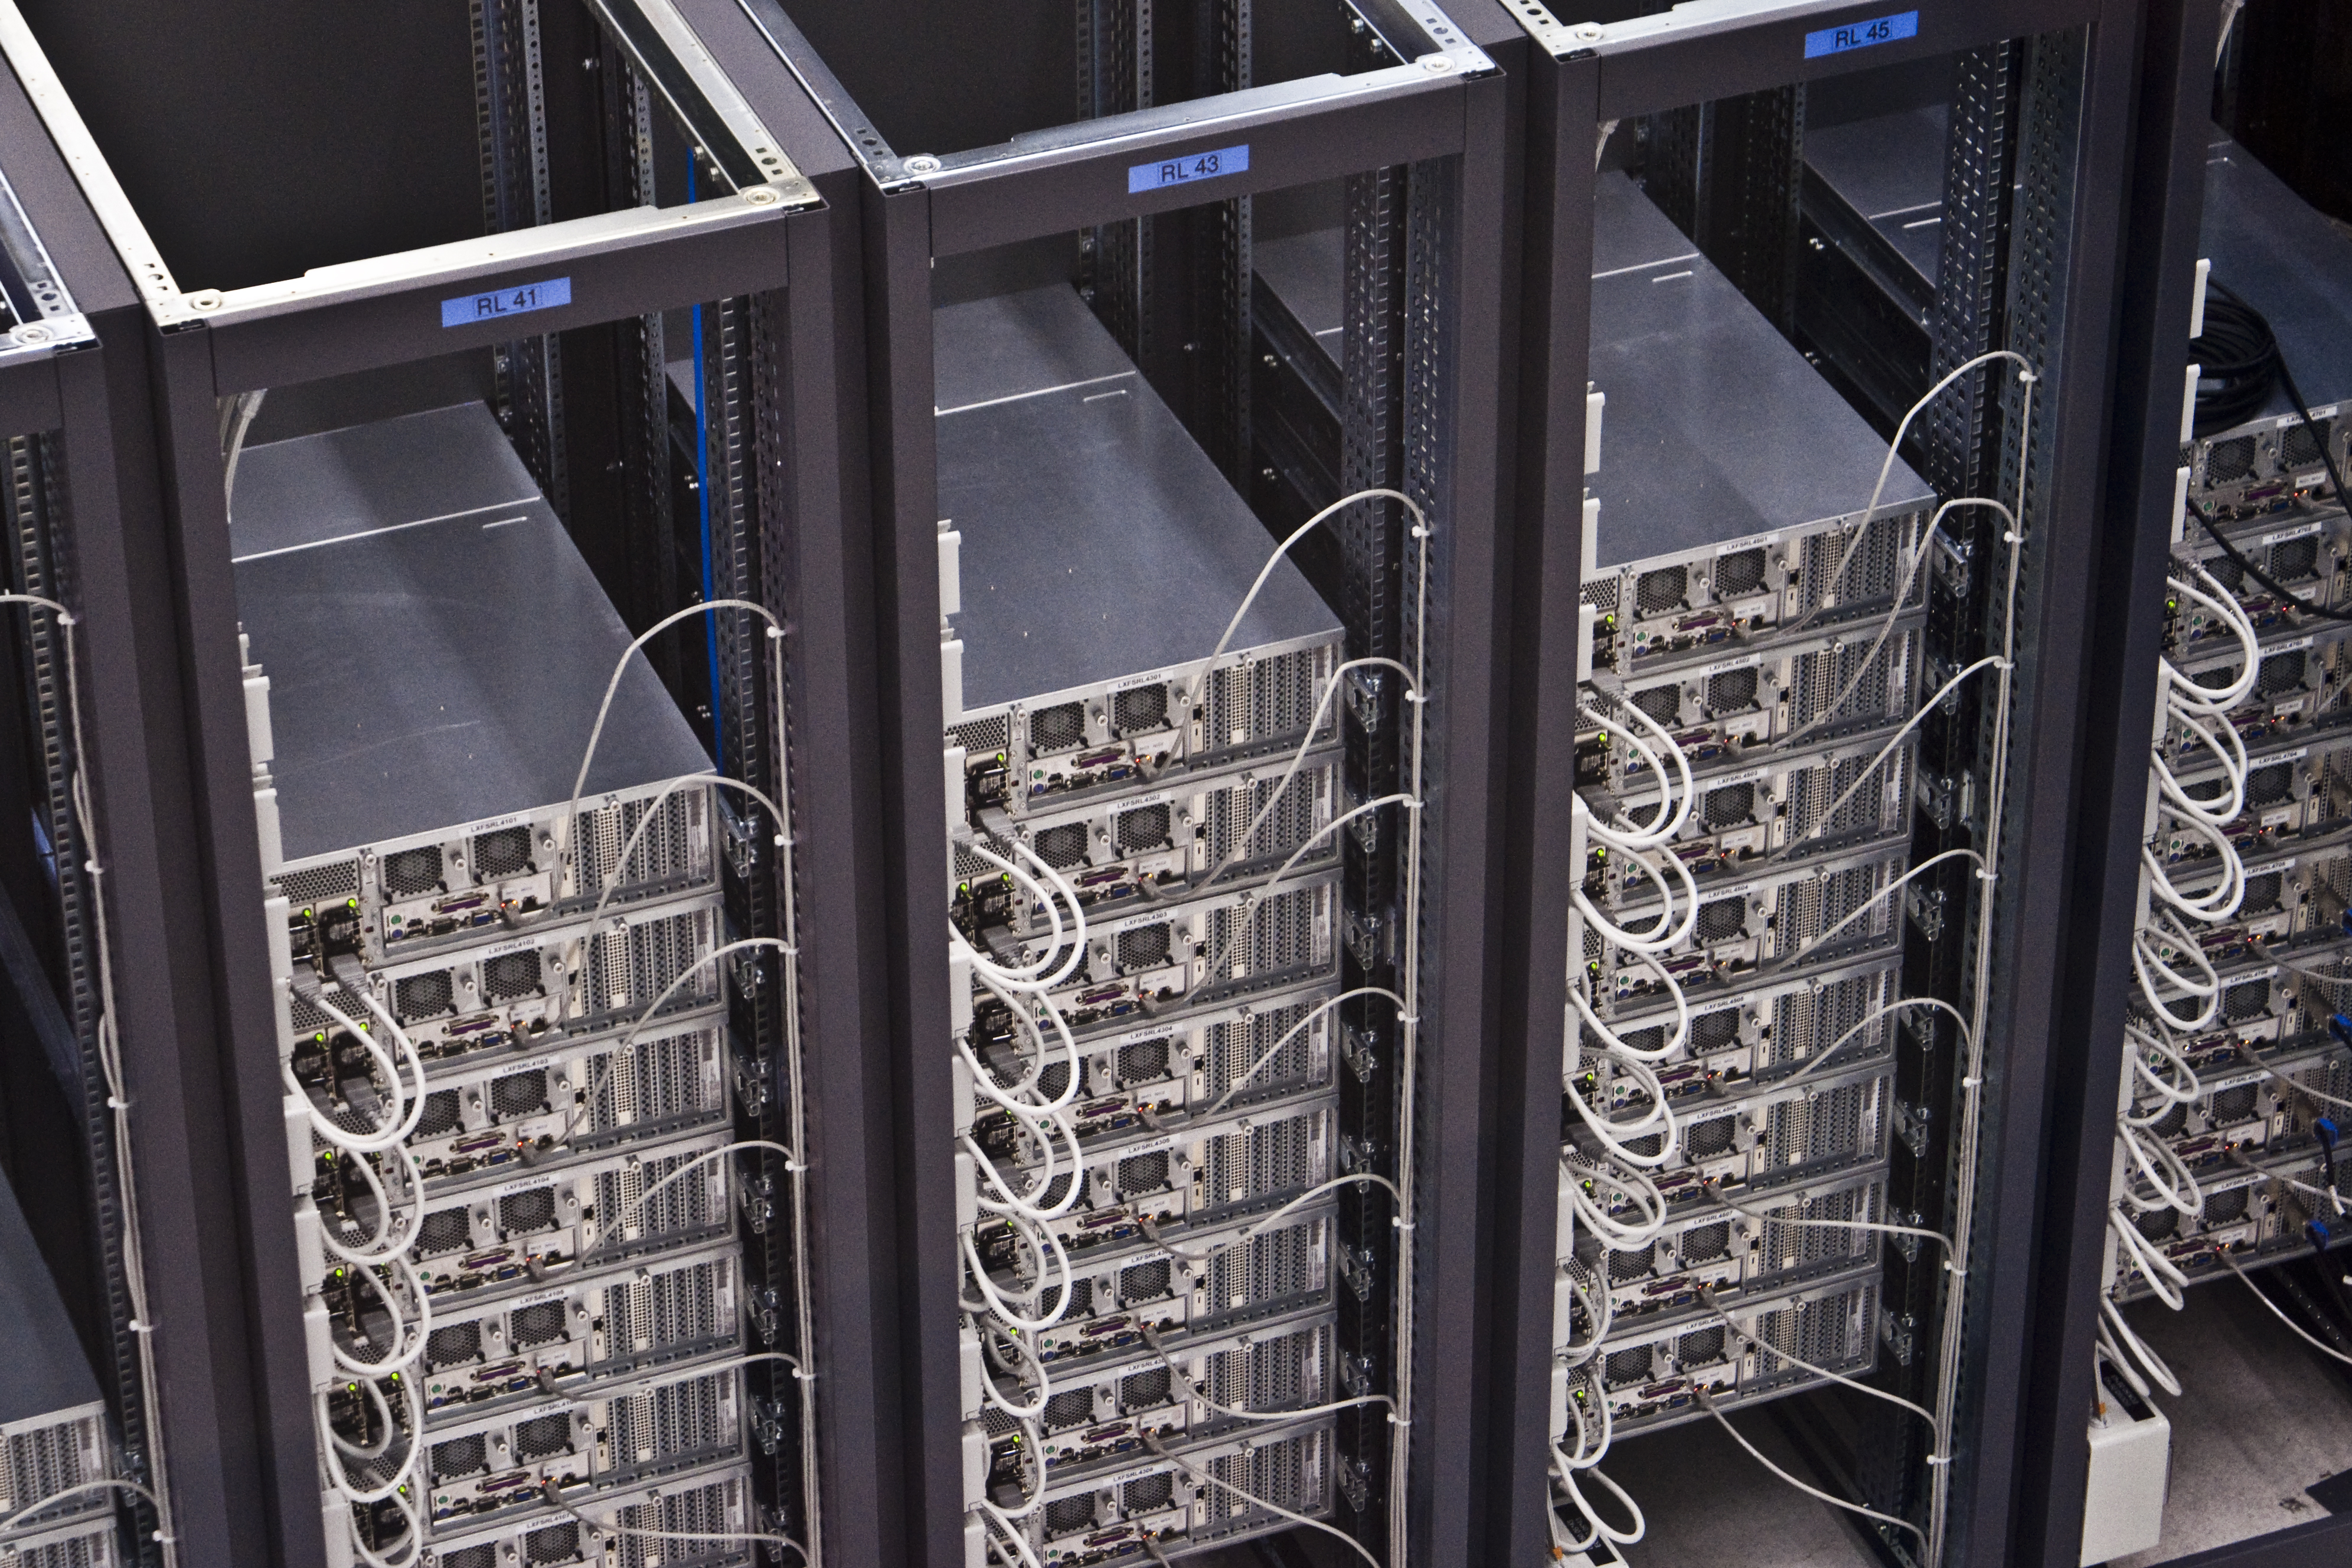
\includegraphics[width=0.8\textwidth]{images/server.jpg}
\note{Nyní několik zástupů serverových programů. Tady těch obrázků bude
výrazně méně, protože programy běžící na serverech většinou nemají žádné hezké
UI, ze kterého se dá udělat screenshot.}
\end{center}\end{frame}


\begin{frame}\begin{center}
\includegraphics[width=0.5\textwidth]{images/mapserver.png}\\
\url{http://mapserver.org}
\note<1>{
MapServer je opět velice starý projekt, který dělá to, jak se jmenuje: vydává
klientům požadovaná geodata podle požadovanvaných parametrů. MapServer obsahuje
rozhraní MapScript, takže jej lze dost modifikovat pomocí různých skriptovacích
jazyků.~\\
~\\
Na MapServeru běží nebo běžela řada veřejných institucí, kdysi to býva
nejrozšířenější open source mapovací software ve veřejné správě.
}
\end{center}\end{frame}

\begin{frame}\begin{center}
\includegraphics[width=0.5\textwidth]{images/geoserver.png}\\
\url{http://geoserver.org}
\note<1>{
GeoServer je v Javě napsaný mapový server, striktně dodržující standardy. Na
rozdíl od MapServeru disponuje webovým grafickým rozhraním. Lze jej do jisté
míry také programátorsky přizpůsobit, děje se tak ale pomocí REST API, a ne na
úrovni programátorských knihoven.
}
\end{center}\end{frame}

\begin{frame}\begin{center}
\includegraphics[width=0.5\textwidth]{images/postgis.png}\\
\url{http://postgis.org}
\note<1>{
    Prostorová data a prostorové funkce jsou zejména v rozšření PostGIS databáze
    PostgreSQL. Postgis je de-facto standardem pro ukládání prostorových dat do
    relační databáze. Další možností je např. spatial lite, které přidává
    prostorové funkce pro databázi spatial lite. ~\\
    ~\\
    Ve světe no-sql databází momentálně vládně mongo-db, ale to jde trochu mimo
    moje zaměření.
}
\end{center}\end{frame}

\begin{frame}\begin{center}
\includegraphics[width=0.7\textwidth]{images/web.jpg}
\note<1>{
Můžete znát například Mapnik nebo jste slyšeli o qgis mapserveru, představený
mapserver a geoserver jsou asi nejdůležitější zástupci tohoto typu software.\\
~\\
Dále bychom se podívaly  na web}
\end{center}\end{frame}

\begin{frame}\begin{center}
\includegraphics<1>[width=0.3\textwidth]{images/ol3.png}
\includegraphics<2>[width=0.4\textwidth]{images/leaflet.png}
\includegraphics<3>[width=0.4\textwidth]{images/d3js.jpg}
\\
\only<1>{\url{http://ol3js.org}}
\only<2>{\url{http://leafletjs.org}}
\only<3>{\url{http://d3js.org}}

\note<1>{
OpenLayers je javascriptová knihovna pro tvorbu mapových aplikací. Je to opravdu
švýcarský nůž, který obsahuje podporu pro všechny myslitelné datové formáty. V
tuto chvíli probíhá přepisování této knihovny na novou verzi pomocí nových
technologií, jako je Google Closure.
}
\note<2>{
    Leaflet stojí technologicky mezi OpenLayer 2 a 3, je to ve srovnání s
    OpenLayers malá knihovna, která umí perfektně zobrazovat mapy a některá
    vektorová data. Leaflet je skvělá volba pro někoho, kdo od aplikace
    nepotřebuje nic moc víc, než data zobrazit a smíří se s některými omezeními
    (jako je např. použ. souř. systém).
}
\note<3>{
    O D3.js toho moc nevím, protože ve své denní práci používám knihovny, které
    mi umožňují stavět cokoliv od aplikací, přes mapové portály až po něco, čemu
    se vznešeně říká Web GIS. D3.js je jiná. \\
    ~\\
    D3.js je knihovna v jazyce javascript, sloužící k manipulaci dokumentů,
    založených na datech. Používá standardní HTML, SVG a CSS techniky a nad nim
    staví celkem slušně schopnou vizualizační platformu.
}
\end{center}\end{frame}

\begin{frame}\begin{center}
\includegraphics[width=0.7\textwidth]{images/library.jpg}
\note<1>{
    Několik zástupců programátorských nástrojů a knihoven, bez kterých by se
    zmiňované nástroje neobešli.
}
\end{center}\end{frame}

\begin{frame}\begin{center}
\includegraphics<1>[width=0.3\textwidth]{images/gdal.png}
\includegraphics<2>[width=0.4\textwidth]{images/proj.png}
\includegraphics<3>[width=0.4\textwidth]{images/geotools.png}
\\
\only<1>{\url{http://gdal.org}}
\only<2>{\url{http://proj.org}}
\only<3>{\url{http://geotools.org}}
\note<1>{
GDAL/OGR je knihovna schopná převézt nepřeberné množství rastrových na
vektorových formátů mezi sebou. Je používána i v proprietárním software ArcGIS.
}
\note<2>{
Knihovna PROJ.4 zase umí pracovat s různými mapovými projekcemi a souř.
systémy. Existuje i verze této knihovny pro jazyk JavaScript, což nám umožuje
tranformovat data mezi souř. systémy přímo na klientovi - v prostředí webového
prohlížeče.
}
\note<3>{
GeoTools dělá to samé pro programovací jazyk Java.
}
\end{center}\end{frame}

\begin{frame}\begin{center}
\includegraphics[width=0.4\textwidth]{images/osgeo.png}\\
\emph{OSGeo Projekt}
\note{
Existuje i řada projektů mimo OSGeo. Mají svou vývojářkou a uživatelskou
komunitu. Asi jste slyšeli o projektu Leaflet, gvSig (ten je v OSGeo
inkubárotru), knihovně D3js pro vykreslování dat na webu.\\
~\\
Řekněte, jaká problematika vás zajímá a já vám řeknu, co bych na to použil. A
nebo ne.
}
\end{center}\end{frame}

\begin{frame}\begin{center}
\includegraphics[width=\textwidth]{images/missing.jpg}
\note{
Může se stát, že na váš úkol neexistuje Open Source odpověď. V tom případě máte
dvě možnosti: zvažte, jestli je ve vašich silách jakkoliv přispět do
existujícího projektu nebo vytvořit nový - je to tak snadné. Nebo jděte do
proprietárního software. Buďte si ale vždy vědomi, proč to děláte a co tím
ztrácíte.
}
\end{center}\end{frame}

\begin{frame}\begin{center}
\includegraphics[width=0.7\textwidth]{images/proprietary_software.png}
\note{
Může se stát, že na váš úkol neexistuje Open Source odpověď. V tom případě máte
dvě možnosti: zvažte, jestli je ve vašich silách jakkoliv přispět do
existujícího projektu nebo vytvořit nový - je to tak snadné. Nebo jděte do
proprietárního software. Buďte si ale vždy vědomi, proč to děláte a co tím
ztrácíte.
}
\end{center}\end{frame}

\begin{frame}\begin{center}
\includegraphics[width=0.7\textwidth]{images/confused.jpg}
\note{
Z toho všeho co říkám si možná říkáte: proč to tedy nikdo nepoužívá, když je to
tak skvělý produkt? Proč není open source software dávno rozšířenější, než jak
to vypadá?\\
~\\
Důvody pro tento stav -- a je jedno jestli je to objektivní fakt nebo subjektivní
pocit -- jsou samozřejmě mnohé a jak už to bývá, mají povahu vnitřní i vnější.
}
\end{center}\end{frame}

\begin{frame}\begin{center}
\includegraphics<1>[width=0.5\textwidth]{images/archim.jpg}
\includegraphics<2>[width=0.7\textwidth]{images/ponorka.png}
\note{
Jako jeden z prvních důvodů (bez nároku na prvenství z hlediska významnosti)
uvedu to, že člověk používá to, co zná. Věřím, že obsahem výuky na
školách ve všech oborech a stupních by měly být především obecně platné
principy, až od nich odvozené konkrétní situace. Učíme obecně Archimedův zákon,
a teprve následně několik jeho praktických aplikací, jako že ve vodě je slon
lehčí nebo}
\note<2>{spolu s inženýry španělského námořnictva, že ponorka, má-li se vynořit,
musí mít především v součtu menší objemovou hustotu, než voda. Proč se ale tento
princip uplatňuje při výuce software jen velice zřídka? Proč výuka počítačí
obecně a GIS konkrétně se téměř bez výjimky provádí na konkrétním jednom
software?
}
\end{center}\end{frame}

\begin{frame}\begin{center}
\includegraphics[width=0.8\textwidth]{images/empty-chair.jpg}
\note{
Dalším důvodem je neexistence jednotného telefonního čísla -- chybí marketingové
oddělení open source GIS, není tu někdo, kdo by zákazníkům vysvětlil proč je
konkrétní produkt ten nejlepší (v absolutním i relativním významu). U open source
software se předpokládá, že jste dospělí, že jste nebo se chcete stát experty a
proto na to, co je pro váš případ to nejlepší si přijdete sami. Open source je
náročný na lidské zdroje, pokud nemáte u sebe někoho dalšího, jste v tom tak
trochu sami, ,,jenom`` s podporou komunity. To může hodně lidí odradit, ale
bylo mnohokrát  ilustrováno, že podpora komunity funguje, první odpověď v mailing
listech bývá u větších projektů v řádu minut.
}
\end{center}\end{frame}

\begin{frame}\begin{center}
\includegraphics[width=0.7\textwidth]{images/market.jpg}
\note{
Dalším důvodem bude roztříštěná nabídka open source software. Jak jsem řekl
dříve, nemáte se moc koho zeptat a ještě ke všemu si musíte vybírat z množství
variant -- sám s tím mám často problém. Provozní výzkum, porovnávání různých
programů a sledování nových je denní chléb. Mám vzít TileCache, MapStach,
GeoServer cache, MapCache? A co je to ten Mapnik? A jaký je rozdíl mezi Leaflet
a OpenLayers? Na tyto otázky získáte nejlépe odpověď tak, že budete číst nebo se
zeptáte někoho, kdo to ví, ale jak jsem již řekl -- ve vašem okolí je většinou
problém najít někoho kdo by to věděl. Nebo snad ne?
}
\end{center}\end{frame}

\begin{frame}\begin{center}
\includegraphics[width=0.7\textwidth]{images/mentors.png}\\
\url{http://gismentors.eu}
\note{
Dalším důvodem je nejednotný systém návazného vzdělávání. Existují spíše
jednotlivci, nabízející školení. Školení jsou ale nejednotná, různá obsahem i
kvalitou. To se snažíme odbourat naším projektem GISMentors
}
\end{center}\end{frame}

\begin{frame}\begin{center}
    \uncover<1->{\includegraphics[width=0.4\textwidth]{images/data-open.jpg}}
    \uncover<2->{\includegraphics[width=0.4\textwidth]{images/mapping-software.jpg}}
    \\
    \uncover<3->{\includegraphics[width=0.4\textwidth]{images/SettingStandard.png}}
    \note{
Otevřený svět Geo* má kromě dvou již zmíněných částí -- totiž Open Data \mynext \\

a Open Source Software \mynext \\

ještě jednu důležitou část, a tou je\\

Open Standards. Tu pro nás zajištuje organizace Open Geospatial Consorcium.
}
\end{center}\end{frame}

\begin{frame}\begin{center}
\includegraphics[width=0.7\textwidth]{images/ogc.png}\\
\url{http://opengeospatial.org}
\note{
OGC je mezinárodní standardizační organizace pro Geo* doménu. Standardizuje
formáty a služby. Její standardy jsou vždy a zásadně otevřené a hlavně, široce
akceptované vývojářskou a uživatelksou komunitou. Možná jste slyšeli o službách
OGC WMS, WFS, WCS nebo WPS a CSW. Tyto služby vám umožňují stahovat mapy,
vektorová a rastrová data, spouštět výpočty  na serverech (nebo jak se dnes
říká, v cloudu) nebo vyhledávat data služby po celém světě. Zdá se vám to příliš
abstraktní?
}
\end{center}\end{frame}

\begin{frame}\begin{center}
\includegraphics[width=0.4\textwidth]{images/inspire-logo.jpg}
\includegraphics[width=0.4\textwidth]{images/open_services.jpg}
\note{
V roce 2007 byla evropskou komisí schválena směrnice INSPIRE, která (velice
zjednodušeně řečeno) popisuje způsob, jakým má veřejná správa umožnit přístup k
datům (nejen, ale zejména) o životním prostředí. Směrnice neříká nic o tom za
jakých právních a finančních podmínek mají být data zveřejněna - nejedná se o
Open Data. Řeší ale technickou a obsahovou stránku věci a ve svých pravidelch
pro implementaci se důrazně opírá právě o standardy OGC.
}
\end{center}\end{frame}

\begin{frame}\begin{center}
    \note{Takže: ve své přednášce jsem mluvil o Open Source, Open Data, Open Standards pro
doménu Geo. Proč jsou skvělé a snad i proč nefungují. Už i u nás a u vás na
Slovensku existují firmy, které nabízejí profesionální služby v této doméně.
Také díky velké finančních krizi posledních let se daří stále častěji firmám z
open soure světa prorážet na komerčním poli.
}
\end{center}\end{frame}

\begin{frame}\begin{center}
\includegraphics[width=0.3\textwidth]{images/dobias.jpg}
\hfill
\includegraphics[width=0.3\textwidth]{images/mitasova.jpg}\\
Martin Dobiáš (QGIS) \hfill Helena Mitášová (GRASS)\\
\includegraphics[width=0.3\textwidth]{images/hofierka.jpg}
\hfill
\includegraphics[width=0.3\textwidth]{images/ivan.png}\\
Jaroslav Hofierka (GRASS) \hfill Ivan Mikčík (GIS.lab)
\note{
Myslím, že i vzhledem k tomu kolik Slovenských vývojářů se pohybuje na open
source GIS scéně, má Slovensko a snad i Česko světlou geo-budoucnost.
}
\end{center}\end{frame}

\begin{frame}\begin{center}
    ?
\note{dotazy?}
\end{center}\end{frame}

\end{document}
